\chapter{CPU部分}

\section{流水线结构}
\subsection{基本单发射结构}
流水线可以将一条指令的指令拆分成多个较小的步骤,每个步骤都可以按照更高的频率运行从而能够提高CPU的最终运行频率。通常可以将指令的执行划分成为5级流水线
\begin{itemize}
	\item \textbf{取指(IF)}:从内存中读取需要执行的指令。
	\item \textbf{译码(ID)}:将指令进行译码。同时读取指令所需要寄存器值,解析指令码中的立即数并进行扩展,对跳转指令给出跳转地址。
	\item \textbf{执行(EX)}:按照译码阶段的指令类型,给出对应结果。
	\item \textbf{访存(MM)}:如果需要访问内存,则在这一阶段进行。
	\item \textbf{回写(WB)}:将运算结果保存到对应寄存器。
\end{itemize}

\begin{figure}[htbp]
	\centering
	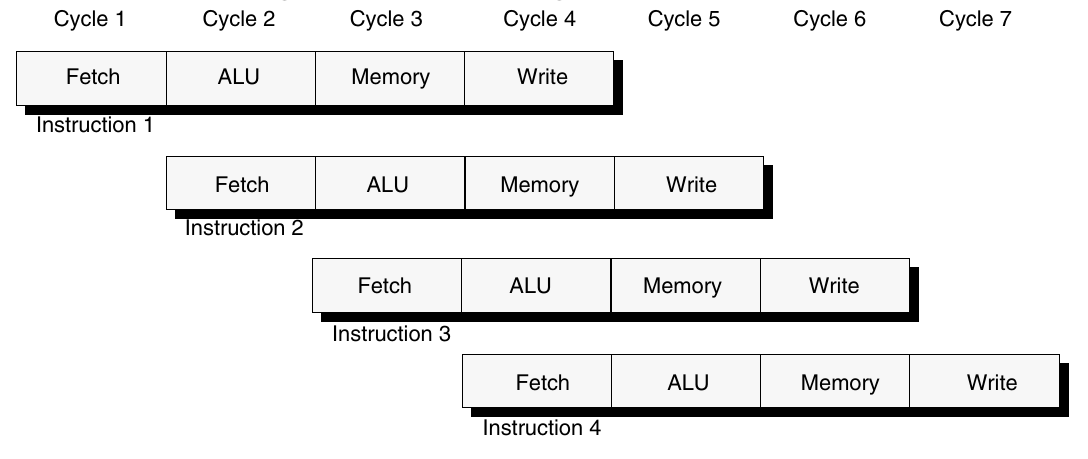
\includegraphics[width=\linewidth]{standard-pipeline.png}
	\caption{标准的流水线结构,图示中没有绘制出译码阶段。}
	\label{fig:standard-pipeline}
\end{figure}

流水线结构本身在带来性能的提升的同时还会带来一部分冒险问题,有以下三种
\begin{itemize}
	\item \textbf{结构冒险}:多条指令对同一资源进行访问。例如访存和取指同时对一个地址进行访问。
	\item \textbf{数据冒险}:流水线内部一条指令依赖于上一条指令的执行结果。
	\item \textbf{控制冒险}:在ID阶段才能确定跳转地址,但IF阶段就需要获取指令。
\end{itemize}

在MIPS架构中,如果按照如上五级流水线结构实现,则不会出现控制冒险。因为对于跳转指令,其下一条指令无论跳转与否均会执行,这样IF阶段获取的指令刚好能够继续指令。

对于数据冒险有两个方法进行解决:

\begin{itemize}
	\item \textbf{数据旁路}:将计算结果直接送到需要的地方。比如将EX阶段的结果直接送到ID阶段。
	\item \textbf{流水线暂停}:插入空指令,暂停流水线的运行。
\end{itemize}

\subsection{双发射流水线的设计}
双发射是指在一个时钟周期内可以执行两条的CPU指令,更一般地,在一个周期同时内执行多条CPU指令的技术叫做超标量技术,其流水线结构如图\ref{fig:superscalar}所示。双发射能够有效地提高CPU的效率,但是它同时也对流水线的设计带来了一定程度的挑战。

\begin{figure}[htbp]
	\centering
	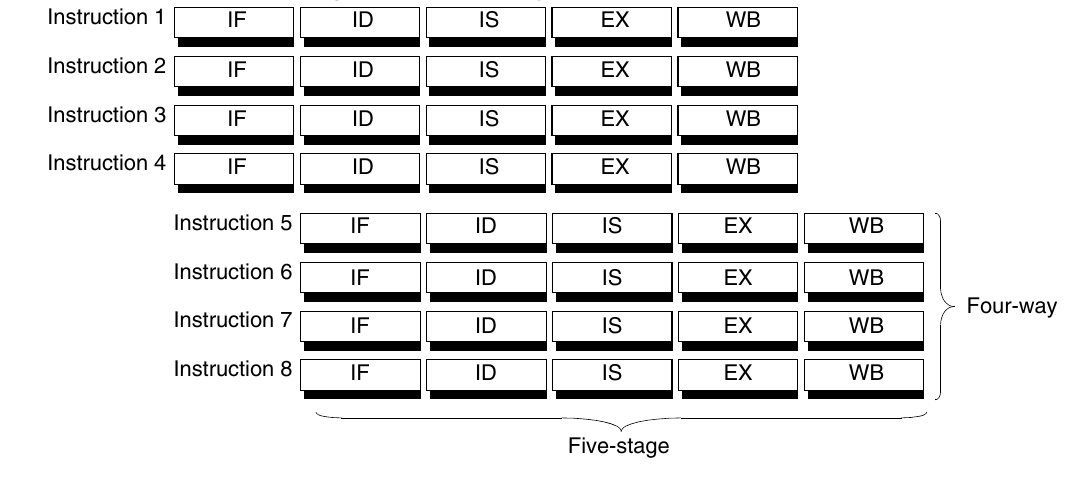
\includegraphics[width=\linewidth]{superscalar.png}
	\caption{超标量流水线结构。}
	\label{fig:superscalar}
\end{figure}

在我们的设计中,对于大部分的指令组合来说流水线是可以两条同时执行的。其结构的设计与标准单发射流水线的主要不同在于IF和ID阶段对指令发射的控制,具体来说有这样两点
\begin{enumerate}
	\item 在IF阶段对PC的修改要保证接下来一个阶段有两条新的指令。因为在取指完成后无法判断这两条指令是否能够一起发射,因此对PC的修改要考虑的是最好情况,也就是它们能够一起发射,但是到了ID阶段,如果这两条指令没有一起发射,那么PC就相当于超前了,这时候就需要针对各个情况进行不同处理。
	\item 在ID阶段译码完成后,需要决定当前的两条指令是否可以同时发射。需要判断的情况较多,例如两条算术指令是否有数据相关,是否是SSNOP这样的特殊指令,是否是分支指令等。
\end{enumerate}

根据ID阶段对何种指令可以同时发射的控制,之后EX和MEM阶段的处理也会有不同之处。这部分内容在我们叙述完这两个部分之后再进行讨论。

在此之前,我们假设从总线获取的指令数据宽度是64位,也就是一次给出一个物理地址,获取64位的数据。

\subsubsection{指令发射控制}
如上所述,在译码阶段需要控制指令是否能够同时发射。如果可以同时发射,那么就把两条指令送给下一阶段,如果判定第二条指令不能够发射,则将其设置为NOP,并且保持第一条不动送给下一阶段。之后执行阶段就可以无需考虑当前两条指令是否是同时发射。

下面是我们实现中\textbf{不能}够同时发射的指令组合,我们称同时发射的两条指令分别为A和B

\begin{itemize}
\item \textbf{Superscalar No Operation} 这是一条类似NOP的指令,其指令代码是SSNOP。在MIPS规范中该条指令必须单独占用一个时钟周期,不能够和其它指令一起发射。

\item \textbf{条件移动指令的数据相关}\ 若指令B为条件移动指令,并且A和B有数据相关,即指令B需要读取指令A需要写的寄存器。由于我们在ID阶段决定寄存器的写信号,需要寄存器的值,而指令B需要的寄存器值在EX阶段才能够获取,因此不同时发射。

\item \textbf{多周期指令的数据相关}\ 对于多周期指令(例如MADDU和FPU指令)如果指令A和B有数据相关,那么不能同时发射。注意对于单周期指令,无论是否有数据相关,我们都可以同时发射。

\item \textbf{分支、特权指令}\ 出于实现方便,指令B不能为分支或者CP0指令。

\item \textbf{延迟槽指令}\ 若指令A为延迟槽,那么下一条指令不能与其一起发射。

\item \textbf{内存相关指令}\ 由于数据总线仅一条,我们只支持A和B中最多有一条访存指令。

\item \textbf{TLB边界指令}\ 如果虚拟地址在TLB边界,其对应的物理地址可能是不连续的,因此此类指令不能够同时发射。因为获取的第二条指令可能无效。这一条是较为特殊的,对之后指令获取的预测部分有较大的影响。
\end{itemize}

\subsubsection{指令获取预测}
指令获取的预测较为复杂,影响该部分的因素主要有二:总线送来的两条物理地址连续的指令是否在虚拟地址上是连续的;上一个周期的两条指令是否同时发射。

预测的原则是需要寻找一个方法,保证在IF阶段对PC的增量进行决策,使得无论当前两条指令是否在ID阶段同时发射,在下一个周期读取得到的两条指令都能够保证双发射的需求。这部分的实现主要是一个有3个不同状态的状态机。

\begin{figure}[htbp]
	\centering
	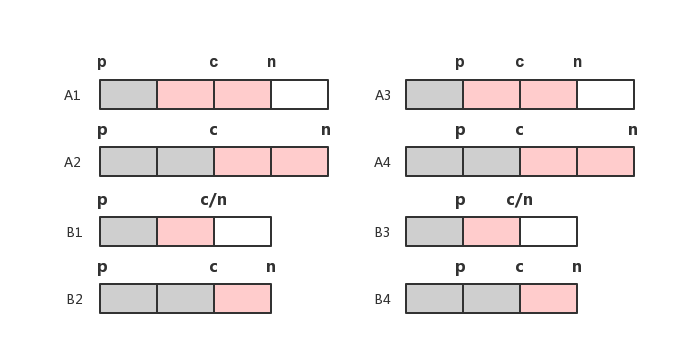
\includegraphics[width=4.3in]{emit-prediction.png}
	\caption{指令获取预测中可能出现的8种情况。p表示上一周期PC的位置,c表示当前PC位置,n表示下一周期PC应该在的位置。灰色部分表示ID发射的指令,红色部分是我们认为可能的接下来一个ID阶段最大发射指令数。c指向的位置右侧两格表示当前IF阶段读取的两条指令。标号为A的四个情况表示当前IF阶段读取到的两条指令没有跨TLB边界,B部分的四个情况表示读取的第二条指令可能不可用,即可能跨TLB边界使得物理地址不连续。}
	\label{fig:emit-prediction}
\end{figure}

该状态机的状态的意义及其对应的转移如下,在每次转移我们可以得到的信息是ID阶段两条指令是否同时发射,以及它们是否在虚拟地址上是连续的(对应跨TLB边界的情况)。对应于当前PC,上一周期的PC和下一周期应该设置的PC值的8种可能如图\ref{fig:emit-prediction}。
\begin{itemize}
	\item \texttt{HARD\_SET} 这表示PC是刚刚经过初始化,或者通过一条转移指令或异常刷新设置而来的,而不是通过PC自身自增得到。
	\item \texttt{MATCH} 表示PC寄存器没有超前于指令的执行,对应于图\ref{fig:emit-prediction}的A3、A4、B3和B4。
	\item \texttt{AHEAD} 表示PC寄存器超前于指令的执行,对应于图\ref{fig:emit-prediction}的A1、A2、B1和B2。
\end{itemize}

状态的转移从图\ref{fig:emit-prediction}基本上可以直接看出。对于情况A1,由于在ID阶段只发射了一条指令,下一阶段如果只发射一条指令,PC会到达当前中间的位置,如果发射两条指令第三个位置,保守地考虑,我们只能对PC增加4。否则如果增加8并且之后只发射一条指令那么下一个阶段的状态PC会领先两条真实执行的指令。已经确定PC增加4后,状态转移自然是当前发射了一条指令那么就转移到AHEAD,发射了两条就转移到MATCH。

对于B2情况,当前最多只有一条指令可用,当然之后最多只能发射一条指令,PC也就只能自增4。再考虑B1,实际上之后最多可以发射两条指令,但是我们为了方便认为之后也最多只能发射一条。那么情况此时PC应该保持不动。

\subsubsection{指令的执行和``数据下推''}
在不考虑数据相关的情况下,指令的执行只需要简单地生成出两个相同的ALU即可。由于我们的设计中,有数据相关的单周期指令也可以同时发射,这样需要进行额外的处理来解决这个相关问题。我们解决的方法类似于``数据前推'',具体的实现是将指令A的ALU计算结果直接通过组合逻辑送到指令B的ALU,再根据情况进行选择。这种实现我们称为``数据下推''。

另外,在访存阶段,由于双发射控制中已经排除了两条指令同时访存的情况,这阶段只需要判断两条指令是否有其一访存再进行对应的处理即可。

\begin{landscape}
\begin{figure}[htbp]
	\centering
	\includegraphics[width=\linewidth]{{datapath_crop.pdf}}
	\caption{CPU数据通路,仅绘制出大致的结构,具体的信号见文字描述。}
	\label{fig:cpu-datapath}
\end{figure}
\end{landscape}
\section{指令集}
下方按照功能划分列举了CPU所支持的MIPS指令,各条指令的具体编码以及功能在MIPS文档中有详细的描述。
\begin{itemize}
	\item \textbf{自陷指令} TGE, TEGU, TLT, TLTU, TEQ, TNE, TGEI, TGEIU, TLTI, TLTIU, TEQI, TNEI
	\item \textbf{分支指令} BLTZ, BGEZ, BLTZAL, BGEZAL, BEQ, BNE, BLEZ, BGTZ, JR, JALR, J, JAL
	\item \textbf{逻辑指令} AND, OR, XOR, ANDI, ORI, XORI, NOR, SLL, SRL, SRA, SLLV, SRLV, SRAV
	\item \textbf{算术指令} ADD, ADDU, SUB, SUBU, ADDI, ADDIU, MUL, MULT, MULTU, DIV, DIVU, MADD, MADDU, MSUB, MSUBU, CLO, CLZ
	\item \textbf{访存指令} SB, SH, SW, SWL, SWR, LB, LH, LWL, LWR, LW, LBU, LHU, LL, SC
	\item \textbf{特权指令} SYSCALL, BREAK, TLBR, TLBWI, TLBWR, TLBP, ERET, MTC0, MFC0
	\item \textbf{条件移动指令} SLT, SLTU, SLTI, SLTIU, MOVN, MOVZ
	\item \textbf{无条件移动指令} LUI, SLT, SLTU, MFHI, MFLO, MTHI, MTLO 
\end{itemize}

\section{协处理器0}
CP0是MIPS规范中必要的一个协处理器,它提供了操作系统所必须的功能抽象,例如异常处理、内存管理和资源访问控制等。

在CP0中有多个32位寄存器,各个寄存器均通过MTC0和MFC0读写。另外,诸如TLBWI、TLBWR和TLBP等特权指令还有异常的发生也有可能会影响其值。

表\ref{table:required_cp0_registers}中列出了必须实现的CP0寄存器。

\begin{table}[!htbp]
    \centering
    \begin{tabular}{|r|l|l|}
    \hline
    \textbf{编号} & \textbf{名称} & \textbf{功能}  \\ \hline
	8 & BadVAddr & 最近发生的与地址相关的异常所对应的地址 \\ \hline
	9 & Count & 计数器 \\ \hline
	11 & Compare & 计时中断控制器 \\ \hline
	12 & Status & 处理器状态及控制 \\ \hline
	13 & Cause & 上一次异常的原因 \\ \hline
	14 & EPC & 上一次异常发生的地址 \\ \hline
	15 & PEId & 处理器版本和标识符 \\ \hline
	16 & Config & 处理器配置 \\ \hline
	30 & ErrorEPC & 上一次异常发生的地址 \\ \hline
    \end{tabular}
    \caption{必要的CP0寄存器}
    \label{table:required_cp0_registers}
\end{table}

为了实现TLB MMU的功能,还需要表\ref{table:mmu_cp0_registers}中所列出的寄存器。

\begin{table}[!htbp]
    \centering
    \begin{tabular}{|r|l|l|}
    \hline
    \textbf{编号} & \textbf{名称} & \textbf{功能}  \\ \hline
	0 & Index & TLB数组的索引 \\ \hline
	1 & Random & 随机数 \\ \hline
	2 & EntryLo0 & TLB项的低位 \\ \hline
	3 & EntryLo1 & TLB项的低位 \\ \hline
	4 & Context & 指向内存中页表入口的指针 \\ \hline
	5 & PageMask & 控制TLB的虚拟页大小 \\ \hline
	6 & Wired & 控制TLB中固定的页数 \\ \hline
	10 & EntryHi & TLB项的高位 \\ \hline
    \end{tabular}
    \caption{MMU所需要的CP0寄存器}
    \label{table:mmu_cp0_registers}
\end{table}

同时,为了支持自定义异常向量,还需要额外实现一个MIPS 32 Rev 2 中的 EBase寄存器。

\section{中断和异常}
\subsection{中断}
MIPS的中断一共有8个,从0开始编号。其中0号中断和1号中断是软件中断,由软件设置Cause寄存器中的对应位来触发。其余6个中断为硬件中断,由外部硬件触发。在实现中,由Count/Compare寄存器组合而成的定时中断的中断号为7。

在我们的实现里,中断信号产生后会在IF阶段捕获,沿着流水线走到MEM阶段后,如果该中断满足触发条件则会触发异常并且进入中断处理程序。中断的触发要求如下条件全部满足:
\begin{enumerate}
	\item \texttt{Status}寄存器中对应的中断被打开;
	\item 全局中断使能,即\texttt{Status.IE}为1;
	\item 当前不在异常处理程序中,即\texttt{Status.EXL}和\texttt{Status.ERL}为0。
\end{enumerate}

\subsection{异常}
MIPS的异常是“精确异常”,也就是在异常发生前的指令都会执行完毕,异常发生之后的指令不会继续执行。在异常发生时,CPU会跳转到对应的异常向量处执行异常处理代码并设置CP0中对应的寄存器记录异常的原因和一些额外的信息,同时还会进入Kernel Mode。处理异常代码的异常向量由“基地址+偏移”来决定,偏移是根据异常来确定的,基地址是由CP0的EBase寄存器决定。

在我们的实现中,在流水的各个阶段产生了异常,不会马上触发,而是被记录下来,顺着流水直到MEM阶段完成后再进行触发。同时,还会考虑双发射两条流水线,优先触发第一条流水线的异常。特别地,异常返回指令ERET被实现为一种特殊的异常,保留到MEM阶段触发。

需要支持的异常在表\ref{table:main-exception}中列出。

\begin{table}[htbp]
	\centering
	\begin{tabular}{|c|c|l|} \hline
		\textbf{异常简称} & \textbf{异常说明} \\ \hline
		Int & 中断  \\ \hline
		Mod & TLB修改异常 \\ \hline
		TLBL & TLB Load异常 \\ \hline
		TLBS & TLB Store异常 \\ \hline
		AdEL & 地址Load异常 \\ \hline
		AdES & 地址Store异常 \\ \hline
		Sys & 系统调用 \\ \hline
		Bp & 断点 \\ \hline
		RI & 保留指令 \\ \hline
		CpU & 协处理器不可用 \\ \hline
		Ov & 算术溢出 \\ \hline
		Tr & 自陷异常 \\ \hline
	\end{tabular}
	\caption{主要支持的异常}
	\label{table:main-exception}
\end{table}
\section{内存管理}
MIPS为操作系统的内存管理提供了较为简单的支持,虚拟地址通过MMU转换为物理地址。MIPS标准对虚拟地址和物理地址的映射如表\ref{tab:virtual-address-space}所示。

\begin{table}[htbp]
	\centering
	\begin{tabular}{|c|c|c|c|} \hline
		\textbf{段} & \textbf{虚拟地址} & \textbf{权限} & \textbf{物理地址} \\ \hline
		kseg3/ksseg & \texttt{0xC000000-0xFFFFFFFF} & Kernel & 由TLB转换 \\ \hline
		kseg1 & \texttt{0xA0000000-0xBFFFFFFF} & Kernel & \texttt{0x00000000-0x1FFFFFFF} \\ \hline
		kseg0 & \texttt{0x80000000-0x9FFFFFFF} & Kernel & \texttt{0x00000000-0x1FFFFFFF} \\ \hline
		useg &  \texttt{0x00000000-0x7FFFFFFF} & User & 由TLB转换 \\ \hline
	\end{tabular}
	\caption{虚拟地址空间}
	\label{tab:virtual-address-space}
\end{table}

具体的地址转换由TLB来完成,TLB可以认为是在CPU内部的地址转换表的高速缓存。具体的内容需要由操作系统来进行填充。如果在TLB中没有找到对应虚拟地址则会触发一个TLB miss异常,操作系统对该异常处理,并且将对应转换表填入TLB中的某一项来完成对地址的转换。我们一共实现了16个TLB项。

\section{静态分支预测}
静态分支预测采用的方案是
\begin{itemize}
	\item 当是无条件跳转指令并且跳转目的地址不存在寄存器中时,认为需要跳转;
	\item 当跳转指令的跳转目标地址小于当前指令地址时,认为需要跳转。这主要是考虑了循环语句;
	\item 当跳转指令的跳转目标地址大于当前指令地址时,认为不需要跳转。这主要考虑了条件语句等。
\end{itemize}

具体的实现方法是在IF阶段进行简单的判断,如果是分支语句则进行预测控制PC的跳转。并且将预测结果往下传入ID阶段,ID阶段再根据预测结果和计算出的该指令的跳转与否进行判断来决定预测是否成功。如果预测失败则需要清空IF阶段的流水,并且将PC设置到真实的分支地址。

因此,最终PC的控制是根据IF阶段分支预测单元、ID阶段分支的反馈信息、双发射控制信息以及上一次的PC地址综合起来计算得出。

\section{浮点运算单元}
MIPS规范中,浮点运算单元(FPU)对应于协处理器1。其共有32个浮点寄存器,由于我们仅支持单精度浮点运算指令,浮点寄存器被实现为32位。浮点数按照IEEE 754标准进行存储。另外,FPU还有一部分特殊的控制寄存器,用于存储FPU的状态信息。其中较为重要的是FPU的比较运算的结果会作为标志位存储在FCSR寄存器的FCC部分中,浮点分支指令会从这个段读取标识位并且进行分支判断。

FPU和CPU之间的数据交互主要有如下几种:
\begin{itemize}
	\item LWC1指令内存中加载数据,SWC1将数据写入内存中;
	\item MFC1指令从CPU的通用寄存器加载数据;MTC1指令将数据写入CPU的通用寄存器;
	\item 浮点分支指令会使得CPU读取\texttt{FCSR.FCC}部分的内容。
\end{itemize}

在我们的实现里FPU直接作为CPU的较为独立的一部分,FPU的流水线就是CPU的流水线。FPU和CPU的数据交互中MFC1指令需要2个周期来完成,这是为了时序的考虑,否则因为数据前推的原因可能会使得组合逻辑过长进而导致CPU频率降低。

另外,我们的FPU也可以双发射,但是与CPU不同的是FPU的算术指令的双发射只能在两条指令内有数据相关的情况下进行。

我们实现的浮点指令主要有:
\begin{itemize}
	\item \textbf{分支指令} C.cond、BC1F、BC1T
	\item \textbf{数据指令} LWC1、SWC1、MFC1、MTC1、CFC1、CTC1
	\item \textbf{算术指令} ABS、ADD、SUB、SQRT、NEG、MUL、DIV
	\item \textbf{舍入指令} ROUND、CEIL、FLOOR、TRUNC、CVT.w、CVT.s
\end{itemize}

	这些指令的具体意义参考MIPS文档。所有算术指令以及CVT.w均按照ROUND模式进行舍入。
\section{代码结构}
CPU部分的代码主要在src/cpu目录下,其主要模块见表\ref{tab:cpu-code-structure}。

同时,由于在流水线各个阶段之中传递的信号太多,我们利用SystemVerilog的packed特性,将公共的信号包装成为一个结构以便于能够简化代码的实现。

\begin{table}
	\centering
	\begin{tabular}{|c|c|} \hline
		cpu\_defs.svh & CPU所需常量、结构定义 \\ \hline
		trivial\_mips.sv & CPU顶层模块 \\ \hline
		ctrl.sv & 流水线暂停和刷新的控制信号 \\ \hline
		hilo.sv & HILO寄存器模块 \\ \hline
		ll\_bit.sv & LLBit寄存器模块 \\ \hline
		regs.sv & CPU通用寄存器模块 \\ \hline
		fpu\_regs.sv & FPU寄存器模块 \\ \hline
		except.sv & 异常请求处理模块 \\ \hline \hline
		if/cpu\_if.sv & IF阶段处理模块 \\ \hline
		if/reg\_pc.sv & PC控制模块  \\ \hline
		if/if\_id.sv & IF/ID数据传输模块 \\ \hline \hline
		id/cpu\_id.sv & ID阶段处理模块 \\ \hline
		id/id\_type\_i/j/r.sv & ID阶段I/J/R型指令译码模块 \\ \hline
		id/fpu\_id.sv & FPU译码模块 \\ \hline
		id/branch.sv & 分支处理模块 \\ \hline
		id/superscalar\_ctrl.sv & 双发射控制模块 \\ \hline
		id/fcsr\_mux.sv & FPU控制寄存器选择模块 \\ \hline
		id/id\_ex.sv & ID/EX数据传输模块 \\ \hline \hline
		ex/cpu\_ex.sv & 单周期指令执行模块 \\ \hline
		ex/ex\_multi\_cycle.sv & 多周期指令执行模块 \\ \hline
		ex/ex\_count\_bit.sv & CLO/CLZ指令执行模块 \\ \hline
		ex/div\_uu.v & DIV指令执行模块 \\ \hline
		ex/fpu\_ex.sv & FPU指令执行模块 \\ \hline
		ex/fpu\_float2int.sv & 浮点转整数指令执行模块 \\ \hline
		ex/ex\_mem.sv & ID/EX数据传输模块 \\ \hline \hline
		mem/cpu\_mem.sv & MEM阶段处理模块 \\ \hline
		mem/mem\_wb.sv & MEM/WB数据传输模块 \\ \hline \hline
		wb/cpu\_wb.sv & WB阶段处理模块 \\ \hline \hline
		cp0/cp0.sv & CP0模块 \\ \hline
		cp0/lfsr.sv & 随机数发生器 \\ \hline
	\end{tabular}
	\caption{CPU部分代码结构。}
	\label{tab:cpu-code-structure}
\end{table}
